\documentclass[12pt,notitlepage,a4paper]{article}
\usepackage{setspace} \doublespacing
\usepackage{courier}
\usepackage{float}
\floatstyle{plaintop}
\restylefloat{table}
\usepackage{ amssymb }
\usepackage{longtable}
\usepackage{rotating}
\usepackage{chngcntr}
\usepackage{soul}
\usepackage{graphicx}
\usepackage{multirow}
\graphicspath{}
\usepackage{tabularx}
\usepackage[top=2cm, bottom=2cm, right=2cm, left=2cm]{geometry}
\renewcommand{\baselinestretch}{1.5}
\usepackage{amsmath, latexsym, amssymb, amsfonts, makeidx, verbatim, epsfig}
\usepackage{graphpap}
\usepackage{multirow}
\usepackage{float}
\usepackage{booktabs}
\usepackage{caption}
\usepackage{subcaption}
\usepackage{longtable}
\usepackage{natbib}
\usepackage{ragged2e}
\bibliographystyle{aer}
\usepackage{tikz}
\usepackage[spanish,english]{babel}
\usepackage{comment}

\hyphenation{me-tho-do-lo-gy ma-xi-mo ba-rril u-ti-li-dad}
\usepackage{graphics}
\usepackage{color}
\definecolor{Blue}{rgb}{0,0,1}
\definecolor{DarkBlue}{rgb}{0,0,0.5}
\definecolor{Red}{rgb}{1,0,0}
\definecolor{Green}{rgb}{0,1,0}
\definecolor{Yellow}{rgb}{1,1,0}
\definecolor{DarkGreen}{rgb}{0,0.4,0}
\definecolor{DarkRed}{rgb}{0.5,0,0}
\definecolor{DarkYellow}{rgb}{0.7,0.7,0}
\usepackage{hyperref}
\hypersetup{colorlinks=true,urlcolor=blue,linkcolor=blue,citecolor=blue}

\interfootnotelinepenalty=10000
\makeatletter
\renewcommand\footnoterule{%
  \vspace{1em}
  \kern-3\p@\hrule\@width.4\columnwidth%
  \kern2.6\p@}
\makeatother


\usepackage[printwatermark]{xwatermark}
\usepackage{xcolor}



\usepackage{lscape}

\begin{document}

\begin{landscape}
\centering\begin{figure}[ht]
\captionsetup{justification=centering}
\caption{The Effect of the Reduction of VAT Rebates in August 2015 - RD Estimates }
\label{fig:rd_robust_2014_0815}
{\centering\begin{tabular}{c c c }
A. Polynomial of Degree 1  & B. Polynomial of Degree 2 & C. Polynomial of Degree 3 \\
\multicolumn{3}{c}{I.  Number of Card Transactions} \\
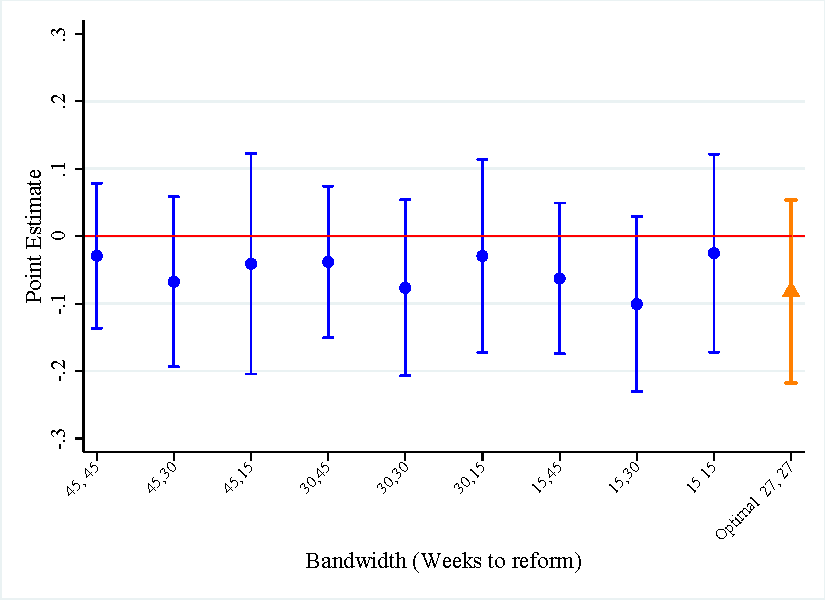
\includegraphics[scale=.4]{output/robust_log_count_trans_1_d_w_0815.pdf} &
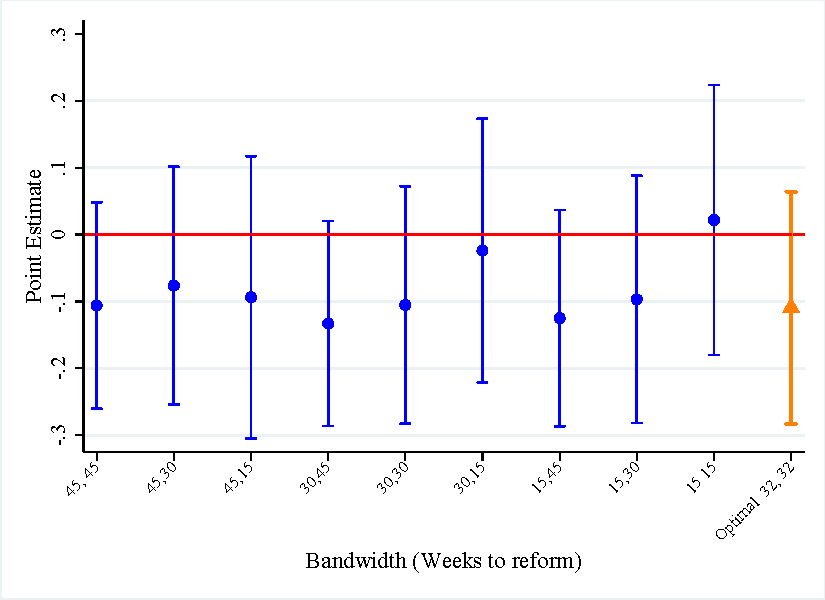
\includegraphics[scale=.4]{output/robust_log_count_trans_2_d_w_0815.pdf} &
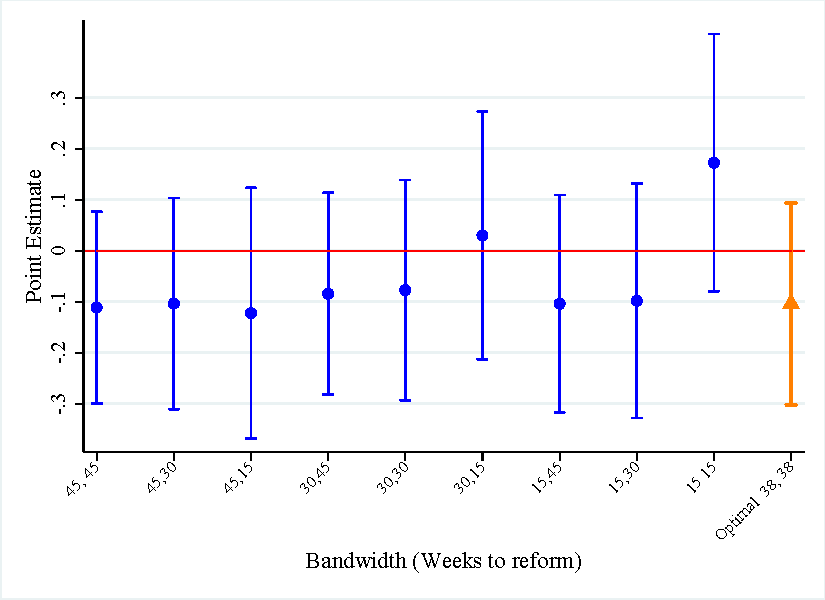
\includegraphics[scale=.4]{output/robust_log_count_trans_3_d_w_0815.pdf} \\
\multicolumn{3}{c}{II.  Volume of Card Transactions} \\
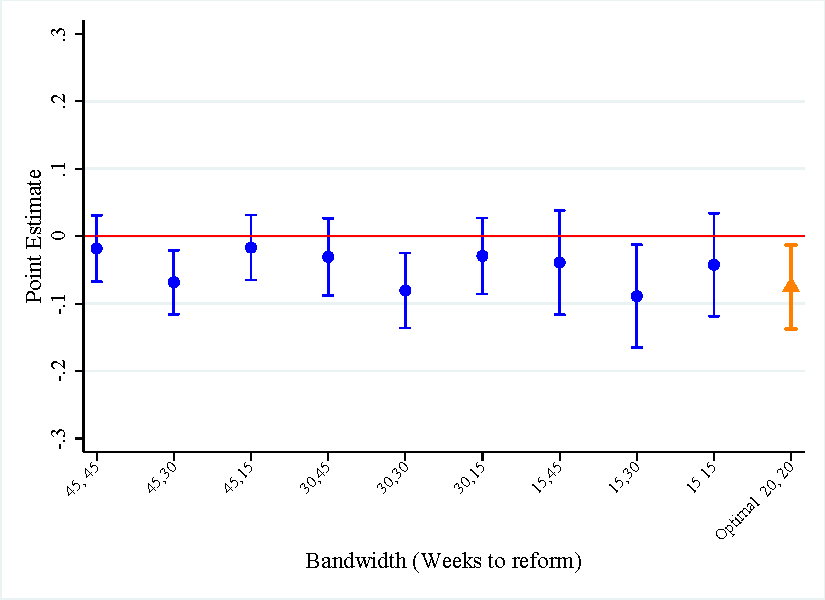
\includegraphics[scale=.4]{output/robust_log_tot_sales_1_d_w_0815.pdf} &
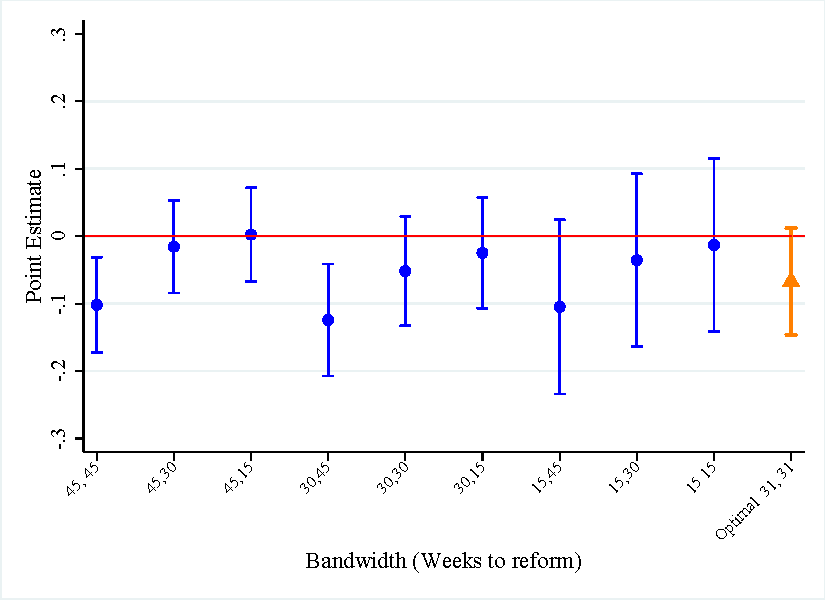
\includegraphics[scale=.4]{output/robust_log_tot_sales_2_d_w_0815.pdf} &
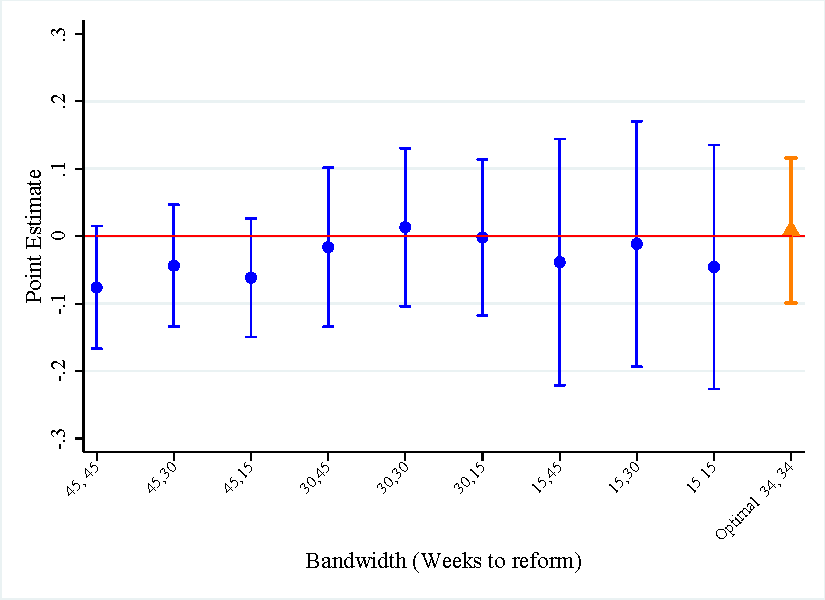
\includegraphics[scale=.4]{output/robust_log_tot_sales_3_d_w_0815.pdf} \\
\multicolumn{3}{c}{III.  Number of POS} \\
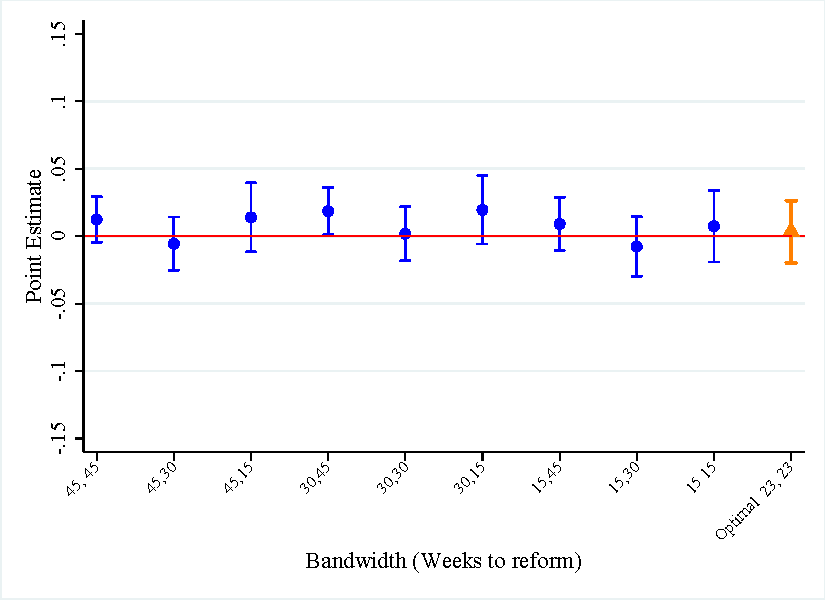
\includegraphics[scale=.4]{output/robust_log_count_pos_total_1_d_w_0815.pdf} &
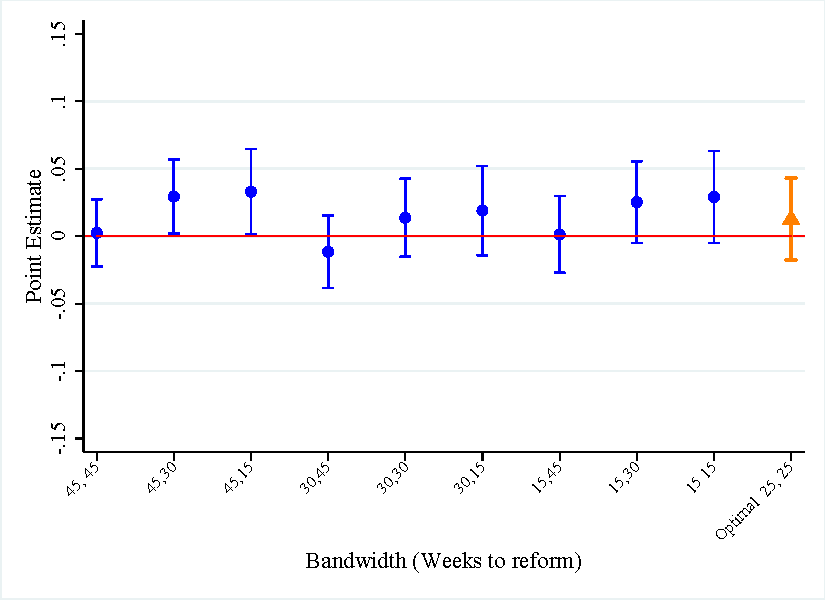
\includegraphics[scale=.4]{output/robust_log_count_pos_total_2_d_w_0815.pdf} &
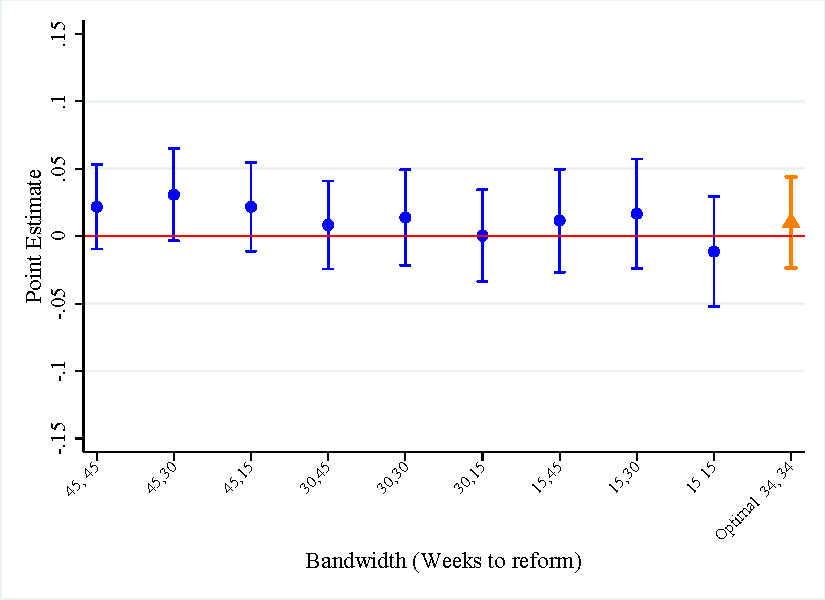
\includegraphics[scale=.4]{output/robust_log_count_pos_total_3_d_w_0815.pdf} \\
\end{tabular}\par}
 	\vspace{.2cm} %\newline 
\begin{spacing}{0.6}
\footnotesize Notes: This Figure  documents the RD estimates around the reduction of the VAT rebates in August 2015, showing that the reduction did not have a statistically significant effect on any of the outcomes.  \ref{sec:rdresults}.
\end{spacing}
\end{figure}
\end{landscape}

\end{document}
